% answers.tex —— 2008 年·普通高等学校招生考试·天津卷·理科 · 参考答案与详细解析片段
% 由 tools/generate_projects.py 依来源总账自 2008/2008_数学真题_天津理_试题.md + 2008/2008_数学真题_天津理_解析正文.md + 2008/2008_数学真题_天津理_答案要点.md 生成，勿手改（改源 MD 后重跑）


\begin{gktip}
固定候选 PDF 仅含题面，无答案、解析和评分标准，原卷亦未标注分值；以下为非官方编者独立推导，官方答案字段为空。来源发布者、出版者、版次与官方身份均未核。
\end{gktip}

\begin{answer}
\gksolhead{1}{}

\textbf{题目}：

$\mathrm i$ 是虚数单位，$\dfrac{\mathrm i^3(\mathrm i+1)}{\mathrm i-1}=$（　）

（A）$-1$

（B）$1$

（C）$-\mathrm i$

（D）$\mathrm i$

\Needspace{4\baselineskip}
\textbf{解析}

\Needspace{5\baselineskip}
计算如下：

\nopagebreak[4]
\[\mathrm i^3=-\mathrm i,\qquad \frac{-\mathrm i(\mathrm i+1)}{\mathrm i-1}=\frac{1-\mathrm i}{\mathrm i-1}=-1.\]

\gkanswer{答案：A。}

\end{answer}
\begin{answer}
\gksolhead{2}{}

\textbf{题目}：

设变量 $x$，$y$ 满足约束条件 $\begin{cases}x-y\geqslant0,\\ x+y\leqslant1,\\ x+2y\geqslant1,\end{cases}$ 则目标函数 $z=5x+y$ 的最大值为（　）

（A）$2$

（B）$3$

（C）$4$

（D）$5$

\Needspace{4\baselineskip}
\textbf{解析}

可行域顶点为 $\left(\dfrac12,\dfrac12\right)$、$\left(\dfrac13,\dfrac13\right)$、$(1,0)$。$z=5x+y$ 取值 $3$，$2$，$5$，故最大值 $5$。

\gkanswer{答案：D。}

\end{answer}
\begin{answer}
\gksolhead{3}{}

\textbf{题目}：

设函数 $f(x)=\sin\left(2x-\dfrac{\pi}2\right)$，$x\in\mathbf R$，则 $f(x)$ 是（　）

（A）最小正周期为 $\pi$ 的奇函数

（B）最小正周期为 $\pi$ 的偶函数

（C）最小正周期为 $\dfrac{\pi}2$ 的奇函数

（D）最小正周期为 $\dfrac{\pi}2$ 的偶函数

\Needspace{4\baselineskip}
\textbf{解析}

\Needspace{5\baselineskip}
计算如下：

\nopagebreak[4]
\[f(x)=\sin\left(2x-\frac{\pi}2\right)=-\cos2x,\]

最小正周期 $\pi$，为偶函数。

\gkanswer{答案：B。}

\end{answer}
\begin{answer}
\gksolhead{4}{}

\textbf{题目}：

设 $a$，$b$ 是两条直线，$\alpha$，$\beta$ 是两个平面，则 $a\perp b$ 的一个充分条件是（　）

（A）$a\perp\alpha$，$b\parallel\beta$，$\alpha\perp\beta$

（B）$a\perp\alpha$，$b\perp\beta$，$\alpha\parallel\beta$

（C）$a\subset\alpha$，$b\perp\beta$，$\alpha\parallel\beta$

（D）$a\subset\alpha$，$b\parallel\beta$，$\alpha\perp\beta$

\Needspace{4\baselineskip}
\textbf{解析}

$b\perp\beta$ 且 $\alpha\parallel\beta$ 给 $b\perp\alpha$；又 $a\subset\alpha$，故 $a\perp b$。

\gkanswer{答案：C。}

\end{answer}
\begin{answer}
\gksolhead{5}{}

\textbf{题目}：

设椭圆 $\dfrac{x^2}{m^2}+\dfrac{y^2}{m^2-1}=1$（$m>1$）上一点 $P$ 到其左焦点的距离为 $3$，到右焦点的距离为 $1$，则 $P$ 点到右准线的距离为（　）

（A）$6$

（B）$2$

（C）$\dfrac12$

（D）$\dfrac{2\sqrt7}7$

\Needspace{4\baselineskip}
\textbf{解析}

\Needspace{5\baselineskip}
由椭圆定义 $2a=3+1=4$，故 $a=2$，即 $m=2$；$b^2=m^2-1=3$，

\nopagebreak[4]
\[c=\sqrt{a^2-b^2}=1,\qquad e=\frac12.\]

\Needspace{5\baselineskip}
点 $P$ 到右焦点的距离为 $1$，由第二定义

\nopagebreak[4]
\[\frac{|PF_{\text{\text{右}}}|}{d}=e\ \Longrightarrow\ d=\frac1{1/2}=2.\]

\gkanswer{答案：B。}

\end{answer}
\begin{answer}
\gksolhead{6}{}

\textbf{题目}：

设集合 $S=\{x\mid|x-2|>3\}$，$T=\{x\mid a<x<a+8\}$，$S\cup T=\mathbf R$，则 $a$ 的取值范围是（　）

（A）$-3<a<-1$

（B）$-3\leqslant a\leqslant-1$

（C）$a\leqslant-3$ 或 $a\geqslant-1$

（D）$a<-3$ 或 $a>-1$

\Needspace{4\baselineskip}
\textbf{解析}

\Needspace{5\baselineskip}
计算如下：

\nopagebreak[4]
\[S=(-\infty,-1)\cup(5,+\infty).\]

\Needspace{5\baselineskip}
$S\cup T=\mathbf R$ 要求 $T=(a,a+8)$ 覆盖 $[-1,5]$：

\nopagebreak[4]
\[a<-1,\qquad a+8>5,\]

故 $-3<a<-1$。

\gkanswer{答案：A。}

\end{answer}
\begin{answer}
\gksolhead{7}{}

\textbf{题目}：

设函数 $f(x)=\dfrac1{1-\sqrt x}$（$0\leqslant x<1$）的反函数为 $f^{-1}(x)$，则（　）

（A）$f^{-1}(x)$ 在其定义域上是增函数且最大值为 $1$

（B）$f^{-1}(x)$ 在其定义域上是减函数且最小值为 $0$

（C）$f^{-1}(x)$ 在其定义域上是减函数且最大值为 $1$

（D）$f^{-1}(x)$ 在其定义域上是增函数且最小值为 $0$

\Needspace{4\baselineskip}
\textbf{解析}

$0\leqslant x<1$ 时 $\sqrt x\in[0,1)$，$1-\sqrt x\in(0,1]$，故 $f(x)\geqslant1$。

\Needspace{5\baselineskip}
反函数：$y=\dfrac1{1-\sqrt x}$，得 $\sqrt x=1-\dfrac1y$，

\nopagebreak[4]
\[f^{-1}(x)=\left(1-\frac1x\right)^2,\qquad x\geqslant1.\]

\Needspace{5\baselineskip}
其导数

\nopagebreak[4]
\[\left(f^{-1}\right)'(x)=2\left(1-\frac1x\right)\cdot\frac1{x^2}>0\quad(x>1),\]

故为增函数；$x\to1^+$ 时趋于 $0$，最小值为 $0$。

\gkanswer{答案：D。}

\end{answer}
\begin{answer}
\gksolhead{8}{}

\textbf{题目}：

已知函数 $f(x)=\begin{cases}-x+1,&x<0,\\ x-1,&x\geqslant0,\end{cases}$ 则不等式 $x+(x+1)f(x+1)\leqslant1$ 的解集是（　）

（A）$\{x\mid-1\leqslant x\leqslant\sqrt2-1\}$

（B）$\{x\mid x\leqslant1\}$

（C）$\{x\mid x\leqslant\sqrt2-1\}$

（D）$\{x\mid-\sqrt2-1\leqslant x\leqslant\sqrt2-1\}$

\Needspace{4\baselineskip}
\textbf{解析}

\Needspace{5\baselineskip}
当 $x<-1$（$x+1<0$）：

\nopagebreak[4]
\[f(x+1)=-(x+1)+1=-x,\]

\nopagebreak[4]
\[x+(x+1)(-x)=x-x^2-x=-x^2\leqslant1,\]

恒成立。

\Needspace{5\baselineskip}
当 $x\geqslant-1$（$x+1\geqslant0$）：

\nopagebreak[4]
\[f(x+1)=(x+1)-1=x,\]

\nopagebreak[4]
\[x+(x+1)x=x^2+2x\leqslant1\ \Longrightarrow\ x^2+2x-1\leqslant0,\]

解得 $-1-\sqrt2\leqslant x\leqslant\sqrt2-1$，与 $x\geqslant-1$ 取交得 $[-1,\sqrt2-1]$。

合得 $x\leqslant\sqrt2-1$。

\gkanswer{答案：C。}

\end{answer}
\begin{answer}
\gksolhead{9}{}

\textbf{题目}：

已知函数 $f(x)$ 是 $\mathbf R$ 上的偶函数，且在区间 $[0,+\infty)$ 上是增函数。令 $a=f\left(\sin\dfrac{2\pi}7\right)$，$b=f\left(\cos\dfrac{5\pi}7\right)$，$c=f\left(\tan\dfrac{5\pi}7\right)$，则（　）

（A）$b<a<c$

（B）$c<b<a$

（C）$b<c<a$

（D）$a<b<c$

\Needspace{4\baselineskip}
\textbf{解析}

\Needspace{5\baselineskip}
计算如下：

\nopagebreak[4]
\[\left|\sin\frac{2\pi}7\right|\approx0.782,\qquad \left|\cos\frac{5\pi}7\right|=\cos\frac{2\pi}7\approx0.623,\]

\nopagebreak[4]
\[\left|\tan\frac{5\pi}7\right|=\tan\frac{2\pi}7\approx1.254.\]

\Needspace{5\baselineskip}
$f$ 为偶函数且在 $[0,+\infty)$ 上递增，故 $f$ 随 $|x|$ 增大而增大，

\nopagebreak[4]
\[b<a<c.\]

\gkanswer{答案：A。}

\end{answer}
\begin{answer}
\gksolhead{10}{}

\textbf{题目}：

有 $8$ 张卡片分别标有数字 $1$，$2$，$3$，$4$，$5$，$6$，$7$，$8$，从中取出 $6$ 张卡片排成 $3$ 行 $2$ 列，要求 $3$ 行中仅有中间行的两张卡片上的数字之和为 $5$，则不同的排法共有（　）

（A）$1344$ 种

（B）$1248$ 种

（C）$1056$ 种

（D）$960$ 种

\Needspace{4\baselineskip}
\textbf{解析}

中间行必须为 $\{1,4\}$ 或 $\{2,3\}$，各有 $2$ 种顺序，共 $2\times2=4$ 种。

\Needspace{5\baselineskip}
固定中间行后，余下 $6$ 个数中选 $2$ 个排成上行、$2$ 个排成下行：共

\nopagebreak[4]
\[\mathrm C_6^2\cdot2!\cdot\mathrm C_4^2\cdot2!=15\cdot2\cdot6\cdot2=360\]

种。其中上行或下行的和为 $5$ 的需排除：余下数中恰有一对和为 $5$（中间行为 $\{1,4\}$ 时为 $\{2,3\}$；为 $\{2,3\}$ 时为 $\{1,4\}$），该对占上行或下行，有 $2\times12=24$ 种，两行共 $48$ 种。

\Needspace{5\baselineskip}
每种中间行有 $360-48=312$ 种，共

\nopagebreak[4]
\[4\times312=1248.\]

\gkanswer{答案：B。}

\end{answer}
\begin{answer}
\gksolhead{11}{}

\textbf{题目}：

$\left(x-\dfrac2{\sqrt x}\right)^5$ 的二项展开式中，$x^2$ 的系数是\gkblank{}。（用数字作答）

\Needspace{4\baselineskip}
\textbf{解析}

\Needspace{5\baselineskip}
通项

\nopagebreak[4]
\[\mathrm C_5^kx^{5-k}\left(-\frac2{\sqrt x}\right)^k=\mathrm C_5^k(-2)^kx^{5-\frac{3k}2}.\]

\Needspace{5\baselineskip}
令 $5-\dfrac{3k}2=2$ 得 $k=2$，系数

\nopagebreak[4]
\[\mathrm C_5^2\cdot4=40.\]

\gkanswer{答案：$40$。}

\end{answer}
\begin{answer}
\gksolhead{12}{}

\textbf{题目}：

一个正方体的各顶点均在同一球的球面上，若该球的体积为 $4\sqrt3\pi$，则该正方体的表面积为\gkblank{}。

\Needspace{4\baselineskip}
\textbf{解析}

\Needspace{5\baselineskip}
计算如下：

\nopagebreak[4]
\[\frac43\pi R^3=4\sqrt3\pi\ \Longrightarrow\ R=\sqrt3.\]

\Needspace{5\baselineskip}
正方体体对角线 $2R=2\sqrt3$，棱长 $a=\dfrac{2\sqrt3}{\sqrt3}=2$，表面积

\nopagebreak[4]
\[6a^2=24.\]

\gkanswer{答案：$24$。}

\end{answer}
\begin{answer}
\gksolhead{13}{}

\textbf{题目}：

已知圆 $C$ 的圆心与抛物线 $y^2=4x$ 的焦点关于直线 $y=x$ 对称。直线 $4x-3y-2=0$ 与圆 $C$ 相交于 $A$，$B$ 两点，且 $|AB|=6$，则圆 $C$ 的方程为\gkblank{}。

\Needspace{4\baselineskip}
\textbf{解析}

抛物线焦点 $(1,0)$ 关于 $y=x$ 的对称点为 $(0,1)$，即圆心。

\Needspace{5\baselineskip}
圆心到直线 $4x-3y-2=0$ 的距离

\nopagebreak[4]
\[d=\frac{|0-3-2|}5=1.\]

\Needspace{5\baselineskip}
弦长 $6$ 给半弦长 $3$，故

\nopagebreak[4]
\[r^2=d^2+3^2=10,\]

圆为 $x^2+(y-1)^2=10$。

\gkanswer{答案：$x^2+(y-1)^2=10$。}

\end{answer}
\begin{answer}
\gksolhead{14}{}

\textbf{题目}：

如图，在平行四边形 $ABCD$ 中，$\overrightarrow{AC}=(1,2)$，$\overrightarrow{BD}=(-3,2)$，则 $\overrightarrow{AD}\cdot\overrightarrow{AC}=$\gkblank{}。
\nopagebreak[4]
\begin{center}% 2008 年天津卷理科第 14 题：平行四边形 ABCD，对角线 AC、BD 已给出向量坐标。
% 来源 PDF：gaokaomath-src/普通高考/2008/2008天津理.pdf
% SHA-256：e2442be3c0179c888e74b31dda58e749b6ab84ac8cccf86eae4677ab3843f48b
% 原页：2008天津理.pdf 第 1 页（A3 三栏）第 2 栏，书页码 487。
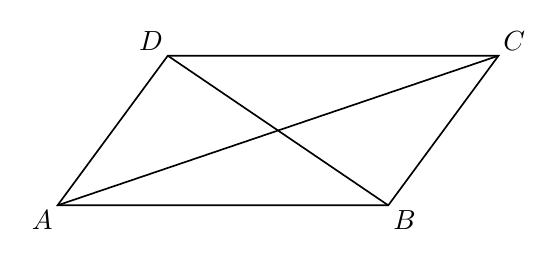
\begin{tikzpicture}[scale=1.0, semithick,
  every node/.style={inner sep=1.5pt}]
  \coordinate (A) at (0,0);
  \coordinate (B) at (4.2,0);
  \coordinate (C) at (5.6,1.9);
  \coordinate (D) at (1.4,1.9);

  \draw (A) -- (B) -- (C) -- (D) -- cycle;
  \draw (A) -- (C);
  \draw (B) -- (D);

  \node[below left] at (A) {$A$};
  \node[below right] at (B) {$B$};
  \node[above right] at (C) {$C$};
  \node[above left] at (D) {$D$};
\end{tikzpicture}
\end{center}
\nopagebreak[4]
\Needspace{4\baselineskip}
\textbf{解析}

\Needspace{5\baselineskip}
设 $\overrightarrow{AB}=\boldsymbol u$，$\overrightarrow{AD}=\boldsymbol v$，则

\nopagebreak[4]
\[\boldsymbol u+\boldsymbol v=(1,2),\qquad \boldsymbol v-\boldsymbol u=(-3,2).\]

\Needspace{5\baselineskip}
两式相加：

\nopagebreak[4]
\[2\boldsymbol v=(-2,4),\qquad \boldsymbol v=(-1,2).\]

\nopagebreak[4]
\[\overrightarrow{AD}\cdot\overrightarrow{AC}=(-1,2)\cdot(1,2)=-1+4=3.\]

\gkanswer{答案：$3$。}

\end{answer}
\begin{answer}
\gksolhead{15}{}

\textbf{题目}：

已知数列 $\{a_n\}$ 中，$a_1=1$，$a_{n+1}-a_n=\dfrac1{3^{n+1}}$（$n\in\mathbf N^*$），则 $\lim\limits_{n\to\infty}a_n=$\gkblank{}。

\Needspace{4\baselineskip}
\textbf{解析}

\Needspace{5\baselineskip}
计算如下：

\nopagebreak[4]
\[a_n=1+\sum_{k=1}^{n-1}\frac1{3^{k+1}}\to1+\frac{1/9}{1-1/3}=1+\frac16=\frac76.\]

\gkanswer{答案：$\dfrac76$。}

\end{answer}
\begin{answer}
\gksolhead{16}{}

\textbf{题目}：

设 $a>1$，若仅有一个常数 $c$ 使得对于任意的 $x\in[a,2a]$，都有 $y\in[a,a^2]$ 满足方程 $\log_ax+\log_ay=c$，这时，$a$ 的取值的集合为\gkblank{}。

\Needspace{4\baselineskip}
\textbf{解析}

\Needspace{5\baselineskip}
$\log_ax+\log_ay=c$ 给 $y=\dfrac{a^c}x$。$x\in[a,2a]$ 时

\nopagebreak[4]
\[y\in\left[\frac{a^c}{2a},\frac{a^c}a\right].\]

\Needspace{5\baselineskip}
要求该区间含于 $[a,a^2]$：

\nopagebreak[4]
\[\frac{a^c}{2a}\geqslant a,\qquad \frac{a^c}a\leqslant a^2,\]

\Needspace{5\baselineskip}
即

\nopagebreak[4]
\[2a^2\leqslant a^c\leqslant a^3.\]

\Needspace{5\baselineskip}
存在 $c$ 需 $2a^2\leqslant a^3$，即 $a\geqslant2$；而 $c$ 唯一需区间退化为一点：

\nopagebreak[4]
\[2a^2=a^3\ \Longrightarrow\ a=2.\]

故 $a$ 的集合为 $\{2\}$。

\gkanswer{答案：$\{2\}$。}

\end{answer}
\begin{answer}
\gksolhead{17}{}

\textbf{题目}：

已知 $\cos\left(x-\dfrac{\pi}4\right)=\dfrac{\sqrt2}{10}$，$x\in\left(\dfrac{\pi}2,\dfrac{3\pi}4\right)$。

（1）求 $\sin x$ 的值；

（2）求 $\sin\left(2x+\dfrac{\pi}3\right)$ 的值。

\Needspace{4\baselineskip}
\textbf{解析}

\Needspace{5\baselineskip}
（1）

\nopagebreak[4]
\[\cos\left(x-\frac{\pi}4\right)=\frac{\sqrt2}2(\sin x+\cos x)=\frac{\sqrt2}{10},\]

\Needspace{5\baselineskip}
故

\nopagebreak[4]
\[\sin x+\cos x=\frac15.\]

\Needspace{5\baselineskip}
设 $s=\sin x$，$c=\cos x$。由 $s^2+c^2=1$ 与 $s+c=\dfrac15$：

\nopagebreak[4]
\[2sc=\frac1{25}-1=-\frac{24}{25},\qquad sc=-\frac{12}{25}.\]

\Needspace{5\baselineskip}
$s$，$c$ 为 $t^2-\dfrac15t-\dfrac{12}{25}=0$ 的两根，即 $25t^2-5t-12=0$：

\nopagebreak[4]
\[t=\frac{5\pm35}{50}=\frac45\ \text{\text{或}}\ -\frac35.\]

\Needspace{5\baselineskip}
$x\in\left(\dfrac{\pi}2,\dfrac{3\pi}4\right)$ 时 $\sin x>0$，故

\nopagebreak[4]
\[\sin x=\frac45,\qquad \cos x=-\frac35.\]

\Needspace{5\baselineskip}
（2）

\nopagebreak[4]
\[\sin2x=2sc=-\frac{24}{25},\qquad \cos2x=c^2-s^2=-\frac7{25}.\]

\nopagebreak[4]
\[\sin\left(2x+\frac{\pi}3\right)=\sin2x\cos\frac{\pi}3+\cos2x\sin\frac{\pi}3
=-\frac{12}{25}-\frac{7\sqrt3}{50}=-\frac{24+7\sqrt3}{50}.\]

\gkanswer{答案：（1）$\dfrac45$；（2）$-\dfrac{24+7\sqrt3}{50}$。}

\end{answer}
\begin{answer}
\gksolhead{18}{}

\textbf{题目}：

甲、乙两个篮球运动员互不影响地在同一位置投球，命中率分别为 $\dfrac12$ 与 $p$，且乙投球 $2$ 次均未命中的概率为 $\dfrac1{16}$。

（1）求乙投球的命中率 $p$；

（2）若甲投球 $1$ 次，乙投球 $2$ 次，两人共命中的次数记为 $\xi$，求 $\xi$ 的分布列和数学期望。

\Needspace{4\baselineskip}
\textbf{解析}

（1）$(1-p)^2=\dfrac1{16}$，故 $1-p=\dfrac14$，$p=\dfrac34$。

\Needspace{5\baselineskip}
（2）设甲命中次数 $X\sim B\left(1,\dfrac12\right)$，乙 $Y\sim B\left(2,\dfrac34\right)$，$\xi=X+Y$。

\nopagebreak[4]
\[P(X=0)=P(X=1)=\frac12,\]

\nopagebreak[4]
\[P(Y=0)=\frac1{16},\quad P(Y=1)=\frac38,\quad P(Y=2)=\frac9{16}.\]

\nopagebreak[4]
\[P(\xi=0)=\frac12\cdot\frac1{16}=\frac1{32},\]

\nopagebreak[4]
\[P(\xi=1)=\frac12\cdot\frac38+\frac12\cdot\frac1{16}=\frac7{32},\]

\nopagebreak[4]
\[P(\xi=2)=\frac12\cdot\frac9{16}+\frac12\cdot\frac38=\frac{15}{32},\]

\nopagebreak[4]
\[P(\xi=3)=\frac12\cdot\frac9{16}=\frac9{32}.\]

\begin{center}
\begin{tabular}{lllll}
\toprule
$\xi$ & $0$ & $1$ & $2$ & $3$ \\
\midrule
$P$ & $\dfrac1{32}$ & $\dfrac7{32}$ & $\dfrac{15}{32}$ & $\dfrac9{32}$ \\
\bottomrule
\end{tabular}
\end{center}

\nopagebreak[4]
\[E\xi=EX+EY=\frac12+\frac32=2.\]

\gkanswer{答案：（1）$p=\dfrac34$；（2）分布列见解析，$E\xi=2$。}

\end{answer}
\begin{answer}
\gksolhead{19}{}

\textbf{题目}：

如图，在四棱锥 $P-ABCD$ 中，底面 $ABCD$ 是矩形。已知 $AB=3$，$AD=2$，$PA=2$，$PD=2\sqrt2$，$\angle PAB=60^\circ$。

（1）证明 $AD\perp$ 平面 $PAB$；

（2）求异面直线 $PC$ 与 $AD$ 所成的角的大小；

（3）求二面角 $P-BD-A$ 的大小。
\nopagebreak[4]
\begin{center}% 2008 年天津卷理科第 19 题：四棱锥 P-ABCD，底面 ABCD 是矩形，
%   AB=3，AD=2，PA=2，PD=2√2，∠PAB=60°。
% 来源 PDF：gaokaomath-src/普通高考/2008/2008天津理.pdf
% SHA-256：e2442be3c0179c888e74b31dda58e749b6ab84ac8cccf86eae4677ab3843f48b
% 原页：2008天津理.pdf 第 1 页（A3 三栏）第 3 栏，书页码 487。
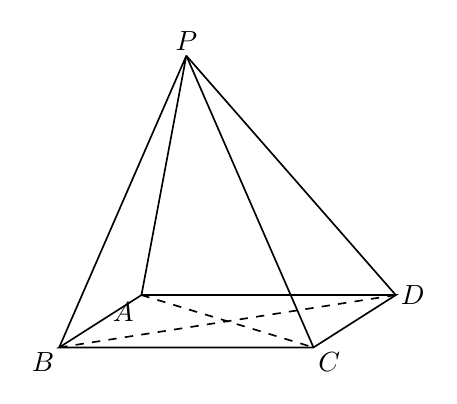
\begin{tikzpicture}[scale=0.95, semithick,
  every node/.style={inner sep=1.5pt}]
  \coordinate (A) at (1.1,0.9);
  \coordinate (B) at (0.0,0.2);
  \coordinate (C) at (3.4,0.2);
  \coordinate (D) at (4.5,0.9);
  \coordinate (P) at (1.7,4.1);

  \draw (A) -- (B) -- (C) -- (D) -- cycle;
  \draw (P) -- (A);
  \draw (P) -- (B);
  \draw (P) -- (C);
  \draw (P) -- (D);
  \draw[dashed] (B) -- (D);
  \draw[dashed] (A) -- (C);

  \node[below left=1pt] at (A) {$A$};
  \node[below left] at (B) {$B$};
  \node[below right] at (C) {$C$};
  \node[right] at (D) {$D$};
  \node[above] at (P) {$P$};
\end{tikzpicture}
\end{center}
\nopagebreak[4]
\Needspace{4\baselineskip}
\textbf{解析}

\Needspace{5\baselineskip}
（1）矩形给 $AD\perp AB$。又

\nopagebreak[4]
\[PA^2+AD^2=4+4=8=PD^2\ \Longrightarrow\ PA\perp AD,\]

故 $AD\perp$ 平面 $PAB$。

\Needspace{5\baselineskip}
（2）以 $A$ 为原点，$AB$ 为 $x$ 轴，$AD$ 为 $y$ 轴。由（1）平面 $PAB$ 为 $y=0$；$PA=2$，$\angle PAB=60^\circ$：

\nopagebreak[4]
\[P(1,0,\sqrt3),\ B(3,0,0),\ C(3,2,0),\ D(0,2,0).\]

\nopagebreak[4]
\[\overrightarrow{PC}=(2,2,-\sqrt3),\qquad \overrightarrow{AD}=(0,2,0),\]

\nopagebreak[4]
\[\cos\theta=\frac4{2\sqrt{11}}=\frac2{\sqrt{11}}.\]

\Needspace{5\baselineskip}
（3）平面 $ABD$ 法向量 $(0,0,1)$；平面 $PBD$：

\nopagebreak[4]
\[\overrightarrow{BD}=(-3,2,0),\quad \overrightarrow{BP}=(-2,0,\sqrt3),\]

\nopagebreak[4]
\[\boldsymbol n=\overrightarrow{BD}\times\overrightarrow{BP}=(2\sqrt3,3\sqrt3,4),\]

\nopagebreak[4]
\[\cos\varphi=\frac4{\sqrt{55}}.\]

故二面角为 $\arccos\dfrac4{\sqrt{55}}$。

\gkanswer{答案：（1）证明见解析；（2）$\arccos\dfrac2{\sqrt{11}}$；（3）$\arccos\dfrac4{\sqrt{55}}$。}

\end{answer}
\begin{answer}
\gksolhead{20}{}

\textbf{题目}：

已知函数 $f(x)=x+\dfrac ax+b$（$x\neq0$），其中 $a$，$b\in\mathbf R$。

（1）若曲线 $y=f(x)$ 在点 $P(2,f(2))$ 处的切线方程为 $y=3x+1$，求函数 $f(x)$ 的解析式；

（2）讨论函数 $f(x)$ 的单调性；

（3）若对于任意的 $a\in\left[\dfrac12,2\right]$，不等式 $f(x)\leqslant10$ 在 $\left[\dfrac14,1\right]$ 上恒成立，求 $b$ 的取值范围。

\Needspace{4\baselineskip}
\textbf{解析}

\Needspace{5\baselineskip}
（1）$f'(x)=1-\dfrac a{x^2}$。由 $f'(2)=1-\dfrac a4=3$ 得 $a=-8$。切点纵坐标 $y=3\times2+1=7$，故

\nopagebreak[4]
\[f(2)=2-4+b=7\ \Longrightarrow\ b=9,\]

\nopagebreak[4]
\[f(x)=x-\frac8x+9.\]

\Needspace{5\baselineskip}
（2）

\nopagebreak[4]
\[f'(x)=\frac{x^2-a}{x^2}.\]

若 $a\leqslant0$，$f'(x)>0$（$x\neq0$），$f$ 在 $(-\infty,0)$、$(0,+\infty)$ 上递增。

若 $a>0$，$f'<0$ 当 $-\sqrt a<x<0$ 或 $0<x<\sqrt a$；$f'>0$ 当 $x<-\sqrt a$ 或 $x>\sqrt a$。故减区间为 $(-\sqrt a,0)$、$(0,\sqrt a)$，增区间为 $(-\infty,-\sqrt a)$、$(\sqrt a,+\infty)$。

\Needspace{5\baselineskip}
（3）需对 $x\in\left[\dfrac14,1\right]$、$a\in\left[\dfrac12,2\right]$：

\nopagebreak[4]
\[b\leqslant10-x-\frac ax.\]

\Needspace{5\baselineskip}
最坏为 $a=2$，故

\nopagebreak[4]
\[b\leqslant10-x-\frac2x\quad\left(\frac14\leqslant x\leqslant1\right).\]

\Needspace{5\baselineskip}
右边导数 $-1+\dfrac2{x^2}>0$（$x<1<\sqrt2$），故在 $x=\dfrac14$ 处取最小值

\nopagebreak[4]
\[10-\frac14-8=\frac74.\]

因此 $b\leqslant\dfrac74$。

\gkanswer{答案：（1）$a=-8$，$b=9$；（2）$a\leqslant0$ 时在 $(-\infty,0)$、$(0,+\infty)$ 上增，$a>0$ 时分区间讨论；（3）$b\leqslant\dfrac74$。}

\end{answer}
\begin{answer}
\gksolhead{21}{}

\textbf{题目}：

已知中心在原点的双曲线 $C$ 的一个焦点是 $F_1(-3,0)$，一条渐近线的方程是 $\sqrt5x-2y=0$。

（1）求双曲线 $C$ 的方程；

（2）若以 $k$（$k\neq0$）为斜率的直线 $l$ 与双曲线 $C$ 相交于两个不同的点 $M$，$N$，线段 $MN$ 的垂直平分线与两坐标轴围成的三角形的面积为 $\dfrac{81}2$，求 $k$ 的取值范围。

\Needspace{4\baselineskip}
\textbf{解析}

\Needspace{5\baselineskip}
（1）$c=3$，渐近线斜率 $\dfrac ba=\dfrac{\sqrt5}2$，故 $b^2=\dfrac54a^2$。由 $a^2+b^2=9$ 得 $a^2=4$，$b^2=5$：

\nopagebreak[4]
\[\frac{x^2}4-\frac{y^2}5=1.\]

\Needspace{5\baselineskip}
（2）设 $l:y=kx+m$，代入双曲线：

\nopagebreak[4]
\[(5-4k^2)x^2-8kmx-4m^2-20=0.\]

\Needspace{5\baselineskip}
两交点要求 $k^2\neq\dfrac54$ 且

\nopagebreak[4]
\[m^2>4k^2-5.\]

\Needspace{5\baselineskip}
中点

\nopagebreak[4]
\[x_0=\frac{4km}{5-4k^2},\qquad y_0=\frac{5m}{5-4k^2}.\]

\Needspace{5\baselineskip}
垂直平分线与两轴截距

\nopagebreak[4]
\[X=x_0+ky_0=\frac{9km}{5-4k^2},\qquad Y=y_0+\frac{x_0}k=\frac{9m}{5-4k^2}.\]

\Needspace{5\baselineskip}
面积条件

\nopagebreak[4]
\[\frac12|XY|=\frac{81|k|m^2}{2(5-4k^2)^2}=\frac{81}2\ \Longrightarrow\ m^2=\frac{(5-4k^2)^2}{|k|}.\]

\Needspace{5\baselineskip}
代入 $m^2>4k^2-5$：$k^2<\dfrac54$ 时恒成立；$k^2>\dfrac54$ 时需

\nopagebreak[4]
\[4k^2-5>|k|\ \Longrightarrow\ |k|>\frac54.\]

\Needspace{5\baselineskip}
故 $k$ 的范围为

\nopagebreak[4]
\[\left(-\infty,-\frac54\right)\cup\left(-\frac{\sqrt5}2,0\right)\cup\left(0,\frac{\sqrt5}2\right)\cup\left(\frac54,+\infty\right).\]

\gkanswer{答案：（1）$\dfrac{x^2}4-\dfrac{y^2}5=1$；（2）$\left(-\infty,-\dfrac54\right)\cup\left(-\dfrac{\sqrt5}2,0\right)\cup\left(0,\dfrac{\sqrt5}2\right)\cup\left(\dfrac54,+\infty\right)$。}

\end{answer}
\begin{answer}
\gksolhead{22}{}

\textbf{题目}：

在数列 $\{a_n\}$ 与 $\{b_n\}$ 中，$a_1=1$，$b_1=4$，数列 $\{a_n\}$ 的前 $n$ 项和 $S_n$ 满足 $nS_{n+1}-(n+3)S_n=0$，$2a_{n+1}$ 为 $b_n$ 与 $b_{n+1}$ 的等比中项，$n\in\mathbf N^*$。

（1）求 $a_2$，$b_2$ 的值；

（2）求数列 $\{a_n\}$ 与 $\{b_n\}$ 的通项公式；

（3）设 $T_n=(-1)^{a_1}b_1+(-1)^{a_2}b_2+\cdots+(-1)^{a_n}b_n$，$n\in\mathbf N^*$，证明 $|T_n|<2n^2$，$n\geqslant3$。

\Needspace{4\baselineskip}
\textbf{解析}

\Needspace{5\baselineskip}
（1）$n=1$：$S_2-4S_1=0$，$S_1=a_1=1$，故 $S_2=4$，

\nopagebreak[4]
\[a_2=S_2-S_1=3.\]

\Needspace{5\baselineskip}
$2a_2$ 为 $b_1$，$b_2$ 的等比中项：

\nopagebreak[4]
\[(2a_2)^2=b_1b_2\ \Longrightarrow\ 36=4b_2,\qquad b_2=9.\]

\Needspace{5\baselineskip}
（2）由 $nS_{n+1}=(n+3)S_n$：

\nopagebreak[4]
\[\frac{S_{n+1}}{S_n}=\frac{n+3}n.\]

\Needspace{5\baselineskip}
累乘：

\nopagebreak[4]
\[S_n=1\cdot\prod_{k=1}^{n-1}\frac{k+3}k=\frac{n(n+1)(n+2)}6.\]

\Needspace{5\baselineskip}
故

\nopagebreak[4]
\[a_n=S_n-S_{n-1}=\frac{n(n+1)}2\quad(n\geqslant2),\]

且 $n=1$ 时也成立。

\Needspace{5\baselineskip}
由 $(2a_{n+1})^2=b_nb_{n+1}$：

\nopagebreak[4]
\[b_nb_{n+1}=(n+1)^2(n+2)^2.\]

\Needspace{5\baselineskip}
结合 $b_1=4=2^2$，归纳得

\nopagebreak[4]
\[b_n=(n+1)^2.\]

\Needspace{5\baselineskip}
（3）$a_k=\dfrac{k(k+1)}2$ 的奇偶性以 $4$ 为周期：$k=1,2,3,4$ 时 $a_k=1,3,6,10$，奇、奇、偶、偶循环。故

\nopagebreak[4]
\[(-1)^{a_k}=-1,-1,1,1,\ldots\]

\Needspace{5\baselineskip}
每四项一组：

\nopagebreak[4]
\[T_{4q}=\sum_{j=0}^{q-1}\left[-b_{4j+1}-b_{4j+2}+b_{4j+3}+b_{4j+4}\right].\]

\nopagebreak[4]
\[- (4j+2)^2-(4j+3)^2+(4j+4)^2+(4j+5)^2=32j+28,\]

\Needspace{5\baselineskip}
故

\nopagebreak[4]
\[T_{4q}=\sum_{j=0}^{q-1}(32j+28)=16q^2+12q.\]

\Needspace{5\baselineskip}
进一步

\nopagebreak[4]
\[T_{4q+1}=-4q-4,\qquad T_{4q+2}=-(16q^2+28q+13),\qquad T_{4q+3}=4q+3.\]

\Needspace{5\baselineskip}
逐类估计（$n\geqslant3$）：

\nopagebreak[4]
\[|T_{4q}|=16q^2+12q<32q^2=2(4q)^2;\]

\nopagebreak[4]
\[|T_{4q+1}|=4q+4<2(4q+1)^2;\]

\nopagebreak[4]
\[|T_{4q+2}|=16q^2+28q+13<32q^2+32q+8=2(4q+2)^2;\]

\nopagebreak[4]
\[|T_{4q+3}|=4q+3<2(4q+3)^2.\]

故对一切 $n\geqslant3$，$|T_n|<2n^2$。

\gkanswer{答案：（1）$a_2=3$，$b_2=9$；（2）$a_n=\dfrac{n(n+1)}2$，$b_n=(n+1)^2$；（3）证明见解析。}

\end{answer}